\documentclass{math}

\usepackage{tikz}

\title{Linear Algebra}
\author{Alvin Lin}
\date{August 2017 - December 2017}

\begin{document}

\maketitle

\section*{Linear Transformations}
\( T:\R^n\to\R^m \) is a transformation if for each \( \vec{x}\in\R^n~\exists!~
T(\vec{x})\in\R^m \). \( Range(T) = Image(T) = \{T(\vec{x})\mid\vec{x}\in\R^n\}
\). \( T:\R^n\to\R^m \) is one-to-one if \( \forall\vec{x},\vec{y}\in\R^n \),
\[ T(\vec{x}) = T(\vec{y}) \longrightarrow \vec{x} = \vec{u} \]
\[ \vec{x} \ne \vec{y} \longrightarrow T(\vec{x}) \ne \vec{y} \]
\( T:\R^n\to\R^m \) is \textbf{onto} (surjective) if \( Range(T) = Codomain(T)
\).

\subsection*{Properties of Linear Transformations}
Let \( T:\R^n\to\R^m \) be a transformation. \( T \) is a linear transformation
if for all \( \vec{u},\vec{v}\in\R^n \) and all scalars \( c,d \):
\begin{enumerate}
  \item \( T(\vec{u}+\vec{v}) = T(\vec{u})+T(\vec{v}) \)
  \item \( T(c\vec{u}) = cT(\vec{u}) \)
  \item \( T(c\vec{u}+d\vec{v}) = cT(\vec{u})+dT(\vec{u}) \)
\end{enumerate}

\subsubsection*{Example}
Suppose \( T:\R^2\to\R^2 \) is defined by:
\[ T\left(\begin{bmatrix}x \\ y\end{bmatrix}\right) = \begin{bmatrix}3y \\
  -4x\end{bmatrix} \]
Verify that \( T \) is linear. Let:
\[ \vec{u} = \begin{bmatrix}x_1 \\ y_1\end{bmatrix} \quad
  \vec{v} = \begin{bmatrix}x_2 \\ y_2\end{bmatrix} \]
\begin{align*}
  T(\vec{u}+\vec{v}) &=
    T\left(\begin{bmatrix}x_1+x_2 \\ y_1+y_2\end{bmatrix}\right) \\
  &= \begin{bmatrix}
    3(y_1+y_2) \\
    -4(x_1+x_2)
  \end{bmatrix} \\
  &= \begin{bmatrix}
    3y_1+3y_2 \\
    -4x_1-4x_2
  \end{bmatrix} \\
  &= \begin{bmatrix}
    3y_1 \\
    -4x_1
  \end{bmatrix}+\begin{bmatrix}
    3y_2 \\
    -4x_2
  \end{bmatrix} \\
  &= T(\vec{u})+T(\vec{v}) \\
  T(c\vec{u}) &= \left(\begin{bmatrix}cx \\ cy\end{bmatrix}\right) \\
  &= \begin{bmatrix}
    3(cy) \\
    -4(cx)
  \end{bmatrix} \\
  &= c\begin{bmatrix}
    3y \\
    -4x
  \end{bmatrix} \\
  &= cT(\vec{u})
\end{align*}
\( T \) satisfies both properties of a linear transformation. To prove a
transformation is not linear, one only needs to find a single counterexample.

\subsubsection*{Example}
Consider \( T:\R^n\to\R^m \) as a linear transformation. What is \( T(\vec{0})
\)?
\begin{align*}
  T(\vec{0}) &= T(\vec{0}+\vec{0}) \\
  &= T(\vec{0})+T(\vec{0}) \\
  \vec{0} &= T(\vec{0})
\end{align*}

\subsection*{Facts about Linear Transformations}
Suppose \( B = \{\vec{v_1},\vec{v_2},\dots,\vec{v_n}\} \) basis for \( R^n \).
Let \( \vec{x}\in\R^n \).
\begin{align*}
  \vec{x} &= \sum_{i=1}^{n}x_1\vec{v_1} \\
  T(\vec{x}) &= T\left(\sum_{i=1}^{n}x_i\vec{v_i}\right) \\
  &= \sum_{i=1}^{n}x_iT(\vec{v_i})
\end{align*}
Let the standard matrix \( A_T \) stand for the linear transformation \( T \):
\begin{align*}
  A_T &= [A] \\
  &= \begin{bmatrix}
    T(\vec{e_1}) & T(\vec{e_2}) & \dots & T(\vec{e_n})
  \end{bmatrix}
\end{align*}
Let \( S:\R^n\to\R^m \) and \( T:\R^m\to\R^k \). The composition of linear
transformations \( T\circ S:\R^n\to\R^k \) is also linear.
\begin{align*}
  [T] &= B \\
  [S] &= A \\
  (T\circ S)(\vec{x}) &= T(S(\vec{x})) \\
  &= T(A\vec{x}) \\
  &= B(A\vec{x}) \\
  &= (BA)\vec{x}
\end{align*}

\subsubsection*{Example}
Define \( \Pi_x:\R^2\to\R^2 \):
\[ \Pi_x\left(\begin{bmatrix}x \\ y\end{bmatrix}\right) = \begin{bmatrix}x \\
  0\end{bmatrix} \]
\( \Pi_x \) is linear. Find \( [\Pi_x] \):
\begin{align*}
  \Pi_x(\vec{e_1}) &= \begin{bmatrix}1 \\ 0\end{bmatrix} \\
  \Pi_x(\vec{e_2}) &= \begin{bmatrix}0 \\ 1\end{bmatrix} \\
  A &= [\Pi_x] = \begin{bmatrix}
    \Pi_x(\vec{e_1}) & \Pi_x(\vec{e_2})
  \end{bmatrix} \\
  &= \begin{bmatrix}
    1 & 0 \\
    0 & 0
  \end{bmatrix}
\end{align*}

\subsection*{Theorems and Definitions}
Let \( T:V\to W \) be linear. \( ker(T) \) is the set of all inputs where the
output through the transformation \( T \) is 0. Then:
\begin{enumerate}
  \item \( ker(T) \) is a subspace of \( V \). Proof:
  \begin{enumerate}
    \item \( T(\vec{0}) = \vec{0} \). Thus \( \vec{0}\in ker(T) \).
    \item Assume \( \vec{u},\vec{v}\in ker(T) \).
    \[ T(\vec{u}+\vec{v}) = T(\vec{u})+T(\vec{V}) = \vec{0}+\vec{0} = \vec{0} \]
    Thus \( \vec{u}+\vec{v}\in ker(T) \).
    \item Assume \( \vec{u}\in ker(T) \) and \( c \) is a scalar.
    \[ T(c\vec{u}) = cT(\vec{u}) = c\vec{0} = \vec{0} \]
  \end{enumerate}
  \item \( Range(T) \) is a subspace of \( W \). Proof:
  \begin{enumerate}
    \item \( T(\vec{0}) = \vec{0} \). So \( \vec{0}\in range(T) \).
    \item Let \( \vec{u},\vec{v}\in range(T) \). Then there exists
    \( \vec{\alpha_u},\vec{\alpha_v} \) such that \( T(\vec{\alpha_u}) =
    \vec{u} \) and \( T(\vec{\alpha_v}) = \vec{v} \).
    \[ \vec{u}+\vec{v} = T(\vec{\alpha_u})+T(\vec{\alpha_v}) =
      T(\vec{\alpha_u}+\vec{\alpha_v}) \]
    So \( \vec{u}+\vec{v}\in range(T) \).
    \item Let \( \vec{u}\in range(T) \). There exists \( \vec{\alpha_u}\in V \)
    such that \( T(\vec{\alpha_u}) = \vec{u} \).
    \[ T(c\vec{\alpha_u}) = cT(\vec{\alpha_u}) = c\vec{u} \]
    Thus \( c\vec{u}\in range(T) \).
  \end{enumerate}
\end{enumerate}

\subsubsection*{Definition}
Let \( T:V\to W \) be linear. The rank of \( T \) is:
\[ dim(range(T)) = rank(T) \]

\subsubsection*{Definition}
The nullity of \( T \) is:
\[ dim(ker(T)) = nullity(T) \]

\subsubsection*{The Rank Theorem}
If \( T:V\to W \) is linear, then:
\[ dim(V) = rank(T)+nullity(T) \]

\subsubsection*{Theorem}
Let \( dim(V) = dim(W) \). Then a linear \( T:V\to W \) is one-to-one if and
only if it is onto.

\subsubsection*{Theorem}
Let \( T:V\to W \) be linear. If \( S = \{\vec{v_1},\dots,\vec{v_2} \} \) is
linearly independent, then \( T(S) = \{T(\vec{v_1}),\dots,T(\vec{v_2})\} \) is
linearly independent in \( W \). Let \( dim(V) = dim(W) = n \). Then a
one-to-one linear transformation \( T:V\to W \) maps a basis for \( V \) to a
basis for \( W \).

\subsubsection*{Theorem}
A linear transformation \( T:V\to W \) is invertible if and only if it is
one-to-one and onto.

\subsubsection*{Example}
Find the kernel and the range of the differential operator \( D:P_3\to P_2 \)
defined by \( D(p(x)) = p'(x) \).
\begin{align*}
  ker(D) &= \{p(x)\in P_3\mid D(p(x)) = 0\} \\
  D(a_0+a_1x+a_2x^2+a_3x^3) &= a_1+2a_2x+3a_3x^2 = 0 \\
  a_1 &= a_2 = a_3 = 0 \\
  ker(D) &= \{a_0\mid a_0\in\R \} \\
  \text{Basis for } ker(D) &= \{1\} \\
  nullity(D) &= 1 \\
  4 &= dim(P_3) = rank(D)+nullity(D) \\
  rank(D) &= 3 \\
  range(D) &= P_2
\end{align*}
\( D \) is onto.

\subsubsection*{Example}
Define \( S:P_1\to R \) by: \( S(p(x)) = \int_{0}^{1}p(x)\diff{x} \). Find the
kernel and range of the transformation.
\begin{align*}
  S(p(x)) &= 0 \\
  S(a+bx) &= 0 \\
  &= \int_{0}^{1}a+bx\diff{x} = \bigg[ax+\frac{bx^2}{2}\bigg]_{0}^{1} =
    a+\frac{b}{2} = 0 \\
  a &= \frac{-b}{2} \\
  ker(D) &= \{-\frac{b}{2}+bx\mid b\in\R\} \\
  \text{Basis for } ker(D) &= \{-\frac{1}{2}+x\} \\
  nullity(D) &= 1 \\
  2 &= dim(P_1) = rank(D)+nullity(D) \\
  rank(D) &= 1 = dim(\R) \\
  range(D) &= \R
\end{align*}
\( D \) is onto.

\subsection*{Isomorphism}
Let \( V,W \) be vector spaces. We say \( T:V\to W \) is an isomorphism if
\( T \) is invertible. We say \( V \) is isomorphic to \( W \). We denote this
as \( V\cong W \). Suppose \( V,W \) have finite dimension. Then \( V\cong W \)
if and only if \( V \) and \( W \) have the same dimension. Example: Is
\( R^4 \) isomorphic to \( M_{22} \)?
\begin{align*}
  dim(\R^4) &= 4 \\
  B &= \left\{
    \begin{bmatrix}1 & 0 \\ 0 & 0\end{bmatrix},
    \begin{bmatrix}0 & 1 \\ 0 & 0\end{bmatrix},
    \begin{bmatrix}0 & 0 \\ 1 & 0\end{bmatrix},
    \begin{bmatrix}0 & 0 \\ 0 & 1\end{bmatrix}
  \right\}\in M_{22} \\
  dim(M_{22}) &= 4 \\
  R^4 &\cong M_{22}
\end{align*}

\subsubsection*{Example}
Is \( P_3 \) isomorphic to \( R^3 \)?
\[ dim(P_3) = 4 \ne dim(R^3) = 3 \]

\subsubsection*{Example}
Suppose \( V,W \) are both n-dimensional. Compute the number of isomorphisms
\( T:V\to W \).
\begin{align*}
  \text{Basis for } V &= \{\vec{v_1},\dots,\vec{v_n}\} \\
  \text{Basis for } W &= \{\vec{w_1},\dots,\vec{w_n}\}
\end{align*}
Number of isomorphisms: \( n! \)

\subsection*{Matrix Associated to a Linear Transformation}
\[ T:\R^n\to\R^m \]
\[ A = [T(\vec{e_1})\mid T(\vec{e_2})\mid\dots\mid T(\vec{e_n})] \]
\[ T:V\to W \quad dim(V) = n \quad dim(W) = m \]
\( V \) has basis \( B = \{\vec{v_1},\dots,\vec{v_n}\} \) and \( W \) has basis
\( G = \{\vec{w_1},\dots,\vec{w_n}\} \).
\begin{center}
  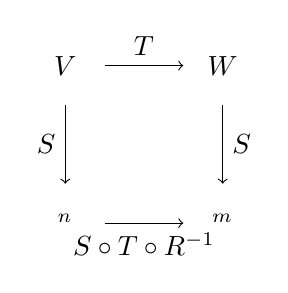
\begin{tikzpicture}
    \node at (0,0) {\( V \)};
    \draw[->] (0.5,0) -- (1.5,0) node[pos=0.5,above] {\( T \)};
    \node at (2,0) {\( W \)};
    \draw[->] (2,-0.5) -- (2,-1.5) node[pos=0.5,right] {\( S \)};
    \node at (2,-2) {\( \R^m \)};
    \draw[->] (0.5,-2) -- (1.5,-2) node[pos=0.5,below]
      {\( S\circ T\circ R^{-1} \)};
    \node at (0,-2) {\( \R^n \)};
    \draw[->] (0,-0.5) -- (0,-1.5) node[pos=0.5,left] {\( S \)};
  \end{tikzpicture}
\end{center}

\subsubsection*{Example}
The transformation \( T:\R^3\to\R^2 \) is linear, defined by:
\[ T\begin{bmatrix}x \\ y \\ z\end{bmatrix} =
  \begin{bmatrix}x-2y \\ x+y-3z\end{bmatrix} \]
The basis for \( \R^3 = \{\vec{e_1},\vec{e_2},\vec{e_3}\} = B \).
The basis for \( \R^2 = \{\vec{e_2},\vec{e_1}\} = G \). Calculate \( T \).

\subsubsection*{Example}
The transformation \( T:P_2\to P_3 \) is defined by:
\[ T(p(x)) = p(2x-1) \]
The basis for \( P_2 = \mathbb{E} = \{1,x,x^2\} \). Calculate
\( [T]_{\mathbb{E}\leftarrow\mathbb{E}} = [T]_{\mathbb{E}} \).
\begin{align*}
  T(1) &= 1 \\
  T(x) &= 2x-1 \\
  T(x^2) &= (2x-1)^2 = 4x^2-4x+1 \\
  [T(1)]_{\mathbb{E}} &= \begin{bmatrix}1 \\ 0 \\ 0\end{bmatrix} \\
  [T(x)]_{\mathbb{E}} &= \begin{bmatrix}-1 \\ 2 \\ 0\end{bmatrix} \\
  [T(x^2)]_{\mathbb{E}} &= \begin{bmatrix}1 \\ -4 \\ 4\end{bmatrix} \\
  [T]_{\mathbb{E}} &= \begin{bmatrix}
    1 & -1 & 1 \\
    0 & 2 & -4 \\
    0 & 0 & 4
  \end{bmatrix}
\end{align*}

\begin{center}
  You can find all my notes at \url{http://omgimanerd.tech/notes}. If you have
  any questions, comments, or concerns, please contact me at
  alvin@omgimanerd.tech
\end{center}

\end{document}
